\part{\trMorse{}理论}%

\chapter*{第一部分引言}\label{mtfh:part1-introduction}
\addcontentsline{toc}{chapter}{第一部分引言}
\markboth{第一部分引言}{第一部分引言}%

\setcounter{figure}{0}
\renewcommand{\thefigure}{\arabic{figure}}

本部分致力于\trMorse{}理论，其首要目标是这样一个\textbf{\trChainComplex}（chain complex）：它由一个\textbf{\trMorseFunction}（Morse function）的\textbf{\trCriticalPoint}（critical point）与一个\trGradient{}场的\trTrajectory{}所定义。

这门理论最初的基石便是如下观察：研究一个（选取得当的）函数，就能得到关于\trManifold\trTopology（topology）的相当精确的信息。最经典的例子——这类例子往往也最有教益——是“\trHeightFunction”（height function）$\RR^3\to\RR$，以及它在\cref{fig:round-sphere} 至 \cref{fig:dented-sphere} 所画的那些不同\trSubmanifold（submanifold）上的限制。在我们要考虑的三种情形里，函数 $f$ 都是 $(x,y,z)\mapsto z$ 的限制。

\begin{figure}[htbp]
\centering
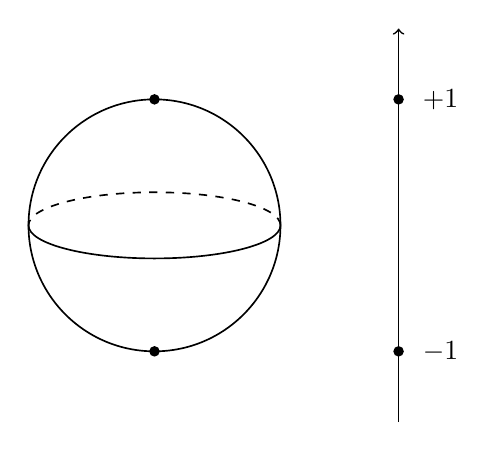
\begin{tikzpicture}[line width=0.6pt]
  \draw (0,0) circle (1.6);
  \draw[dashed] (1.6,0) arc (0:180:1.6 and 0.42);
  \draw (-1.6,0) arc (180:360:1.6 and 0.42);
  \fill (0,1.6) circle (1.9pt);
  \fill (0,-1.6) circle (1.9pt);
  \draw[->] (3.1,-2.5) -- (3.1,2.5);
  \fill (3.1,1.6) circle (1.9pt);
  \node[right] at (3.28,1.6) {$+1$};
  \fill (3.1,-1.6) circle (1.9pt);
  \node[right] at (3.28,-1.6) {$-1$};
\end{tikzpicture}
\caption{圆\trSphere}
\label{fig:round-sphere}
\end{figure}

第一幅图（\cref{fig:round-sphere}）画的是“圆”\trSphere，也就是单位\trSphere
\[
S^2=\bigl\{(x,y,z)\in\RR^3 \bigm| x^2+y^2+z^2=1\bigr\}\text{。}
\]

\textbf{\trLevelSet}（level set）$f^{-1}(a)$ 为
\[
\left\{
\begin{array}{ll}
\varnothing & \text{若 } a<-1 \\
\text{一个点} & \text{若 } a=-1 \\
\text{一个圆} & \text{若 } -1<a<1 \\
\text{一个点} & \text{若 } a=1 \\
\varnothing & \text{若 } a>1\text{。}
\end{array}
\right.
\]

沿着函数的值向上走，我们注意到：各\trLevelSet{}都保持同一种\trTopology，直到遇上某处变故，\trTopology{}在此改变，随后便保持不变，直到下一处变故为止。

同样的情形也适用于“\trSublevelSet”（sublevel set），即位于给定水平之下的部分。它们起初为空，接着（短暂地）是一个点，然后是一个\trDisk，最后是整个\trSphere。

这些变故就是函数的\textbf{\trCriticalValue}（critical value），它们对应于\trCriticalPoint——即 $f$ 的\trDifferential{}为零、\trTangentPlane{}呈水平的那些点，也就是\trSphere{}的北极与南极。当然，南极是函数的最小值，北极则是其最大值。

\begin{figure}[htbp]
\centering
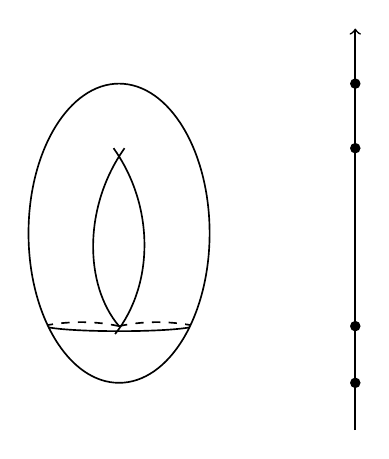
\begin{tikzpicture}[line width=0.6pt]
  \draw (0,0) ellipse (1.15 and 1.9);
  \draw[dashed] (0,-1.18) .. controls (-0.30,-1.115) and (-0.60,-1.115) .. (-0.90,-1.165);
  \draw[dashed] (0,-1.18) .. controls (0.30,-1.115) and (0.60,-1.115) .. (0.90,-1.165);
  \draw (-0.90,-1.195) .. controls (-0.55,-1.26) and (0.55,-1.26) .. (0.90,-1.195);
  \draw (0.07,1.08) .. controls (-0.45,0.35) and (-0.45,-0.65) .. (0,-1.18);
  \draw (-0.07,1.08) .. controls (0.45,0.35) and (0.45,-0.65) .. (-0.05,-1.28);
  \draw[->] (3,-2.5) -- (3,2.6);
  \fill (3,1.9) circle (1.9pt);
  \fill (3,1.08) circle (1.9pt);
  \fill (3,-1.18) circle (1.9pt);
  \fill (3,-1.9) circle (1.9pt);
\end{tikzpicture}
\caption{\trTorus}
\label{fig:torus}
\end{figure}

下一幅图（\cref{fig:torus}）中\trTorus{}的情形类似，只不过现在出现了一些并非函数\trExtremum{}点的\trCriticalPoint，即两个“\trSaddlePoint”（saddle point）。与之相应的\trLevelSet{}是一些呈 8 字形的曲线（图中描出了其中一条），因而不再是\trSubmanifold。至于\trRegular{}的、非临界的\trLevelSet，则由于\trSubmersion{}定理（submersion theorem）而必定都是\trSubmanifold。

这门理论最早的结果之一，是一个归功于\trReeb{}的定理（至少对\trMorseFunction{}而言）。我们将在本部分中证明它。该定理断言：若一个\trCompact\trManifold{}上存在只含两个\trCriticalPoint{}的函数，则它与\trSphere\trHomeomorphic。当然，\trSphere{}上也存在\trCriticalPoint{}更多的函数。

\begin{figure}[htbp]
\centering
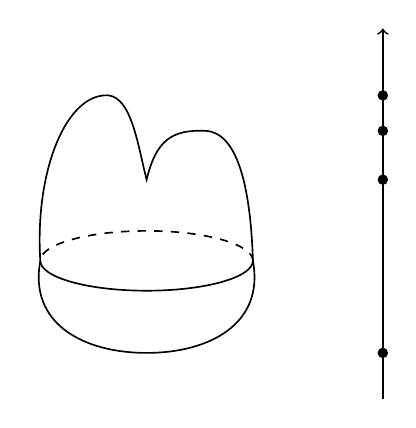
\begin{tikzpicture}[line width=0.6pt]
  \draw[dashed] (1.35,-0.55) arc (0:180:1.35 and 0.38);
  \draw (-1.35,-0.55) arc (180:360:1.35 and 0.38);
  \draw (-1.35,-0.55) .. controls (-1.5,-1.35) and (-0.8,-1.72) .. (0,-1.72)
        .. controls (0.8,-1.72) and (1.5,-1.35) .. (1.35,-0.55);
  \draw (-1.35,-0.55) .. controls (-1.42,0.55) and (-1.05,1.5) .. (-0.55,1.55)
        .. controls (-0.2,1.6) and (-0.12,0.95) .. (0,0.48)
        .. controls (0.12,0.98) and (0.32,1.12) .. (0.75,1.1)
        .. controls (1.15,1.08) and (1.32,0.4) .. (1.35,-0.55);
  \draw[->] (3,-2.3) -- (3,2.4);
  \fill (3,1.55) circle (1.9pt);
  \fill (3,1.1) circle (1.9pt);
  \fill (3,0.48) circle (1.9pt);
  \fill (3,-1.72) circle (1.9pt);
\end{tikzpicture}
\caption{另一个\trSphere}
\label{fig:dented-sphere}
\end{figure}

第三幅图（\cref{fig:dented-sphere}）正是为说明这一点而设。由于它容易想象，我们保留了“同一个”\trHeightFunction，而在\trSphere{}上“压出一个凹坑”。于是，这个\trSubmanifold{}显然仍与\trSphere\trDiffeomorphic，但函数现在有了两个局部极大值和一个\trSaddlePoint。注意，新函数\trCriticalPoint{}个数的奇偶性与原来那个函数相同。若假设这些\trCriticalPoint\trNondegenerate（nondegenerate）（这是一条重要性质，将在后文定义（而且我们图中的\trCriticalPoint{}都满足它）），那么\trCriticalPoint{}的个数模 2 便等于\trManifold{}的\trEulerCharacteristic（Euler characteristic）——一个不依赖于函数、只依赖于\trManifold{}的\trInvariant。

\trWitten{}的\trTrajectory{}空间概念使我们得以给出一个更精细的\trInvariant。显然，\trTorus{}与\trSphere{}是极不相同的两个\trManifold，即便二者都有含四个\trNondegenerate\trCriticalPoint{}的函数。这一\trInvariant{}就是如今人们所称的\trManifold{}的\textbf{\trMorseHomology}（Morse homology）$HM_k(V)$。它是某个\trChainComplex{}的\trHomology，这个\trComplex{}即\textbf{\trMorseComplex}（Morse complex）：由一个\trMorseFunction{}的\trCriticalPoint{}出发，“计数”其沿一个连接这些\trCriticalPoint{}的\trVectorField{}的\trTrajectory，由此构造而成……这些\trTrajectory，就是函数的\trGradient{}的\trTrajectory（相对于某个\trMetric{}而言）。就\trHeightFunction（连同\trEuclidean\trMetric）而言，不妨把这些\trTrajectory{}想成水滴沿曲面从一个\trCriticalPoint{}流到另一个\trCriticalPoint{}的轨迹。

归根结底，这一\trHomology{}只依赖于\trManifold（的\trDiffeomorphic{}型）。我们刚刚就某某\trManifold{}上\trCriticalPoint{}个数所发的议论，可以用著名的“\trMorse{}不等式”（Morse inequalities）来表述：\trManifold{}上一个\trMorseFunction{}的\textbf{\trIndex}（index）为 $k$ 的\trCriticalPoint{}个数 $c_k$ 满足
\[
c_k\geq \dim HM_k(V)\text{。}
\]

因此，让这些对象来做本书第一部分的主题，实在是再自然不过了。

\renewcommand{\thefigure}{\thechapter.\arabic{figure}}
